\chapter{Présentation du cadre du projet}
\setlength{\intextsep}{6pt}
\setlength{\textfloatsep}{8pt}
\setlength{\floatsep}{6pt}
\setlength{\abovecaptionskip}{3pt}
\setlength{\belowcaptionskip}{1pt}
\setlength{\LTpre}{3pt}
\setlength{\LTpost}{3pt}

\newpage

\section{Introduction}
Ce premier chapitre comportera plusieurs parties dont on peut citer l’organisme d’accueil, la 
problématique du projet, la solution proposée ainsi que notre méthodologie adoptée pour le développement de ce projet.

\section{Présentation de l'organisme d'accueil}
Notre projet se déroule au sein de l’entreprise UNIBRO Distribution Plus, une société spécialisée dans la distribution de produits alimentaires et de grande consommation. Elle se distingue par son organisation logistique, son professionnalisme et sa capacité à répondre efficacement aux besoins du marché. UNIBRO Distribution Plus s’engage à assurer un service fiable, basé sur la qualité, la rapidité et la satisfaction de ses partenaires commerciaux.\cite{ref1}
\begin{figure}[H]
  \centering
    
\includegraphics[scale=0.3]{projet/images/logo_unibro-removebg-preview}
  \caption{Logo de la société UNIBRO Distribution Plus}
\end{figure}
\subsection{Domaines d’activités}
UNIBRO Distribution Plus se spécialise dans les domaines suivants :
\begin{itemize}[label=$\rightarrow$]
\item 
 Distribution de produits : Approvisionnement et distribution de produits alimentaires et de grande consommation.
\item 
 Logistique : Gestion du transport, du stockage et de la livraison des marchandises.
\item 
 Gestion commerciale : Relations avec les fournisseurs et les clients, suivi des commandes et des ventes.
\item Service client : Satisfaction des partenaires commerciaux et respect des délais de livraison.
\end{itemize}

\section{Contexte du projet}
Dans cette partie, nous décrivons l'étude de l'existant, les limites ainsi que la solution proposée.
\subsection{Etude de l'existant}
Cette section présente une analyse du système existant de gestion du pointage et des procédures RH, en mettant en évidence ses principales caractéristiques ainsi que ses limites. 
\subsubsection{Description de l'existant}
Le système actuel de gestion du pointage et des procédures RH repose sur des méthodes traditionnelles :
\begin{itemize}
\item Les registres manuels (feuilles de présence) : Les employés signent un document papier à l’arrivée et au départ.

\item  Les systèmes à badges (RFID/Magnétiques) : L’identification repose sur la possession d’une carte que l’employé passe devant un lecteur.

\item L’authentification par codes (PIN) : L’employé saisit un code personnel sur un clavier numérique.
\item Justification d’absence physique : Les justificatifs sont remis manuellement sans dépôt ni archivage numérique.
\item Gestion traditionnelle des primes : L’attribution et le suivi des primes sont effectués manuellement sans consultation numérique pour les employés.
\item Absence de consultation du salaire mensuel : Les employés ne peuvent pas vérifier le statut de leur salaire du mois en cours.

\end{itemize}

\subsubsection{Critique de l'existant et problématique}
Nous citons ci-dessous quelques problèmes liés au système existant :
%===========utiliser une liste à puces simple 
\begin{itemize}
 \item  Erreur humaine : saisie manuelle sujette à des oublis ou des erreurs.

\item Fraude : possibilité de pointage pour un autre employé.

\item Pas de suivi en temps réel : impossibilité de visualiser immédiatement la présence ou l’absence.

\item Gestion lourde : centralisation et analyse des données complexes et fastidieuses..
\item Procédures administratives lentes dues à l’utilisation de documents papier. 
\item Manque de transparence pour les employés concernant les congés, absences, primes et salaires. 
\item Risque de perte ou de détérioration des documents physiques.
\end{itemize}

\subsection{Solution proposée}
Afin de résoudre le problème mentionné plus haut lors de ce projet de fin d'études,
nous allons nous concentrer sur la réalisation d'un logiciel intelligent de gestion des ressources humaines de pointage automatique avec reconnaissance faciale.
Cela aidera à créer un emplacement centralisé pour organiser toute information relative à la gestion des données de présence de nos employés.
Les employés du département de gestion des ressources humaines auront l'opportunité de recevoir des rapports détaillés en peu de temps, parmi lesquels ils seront capables de suivre l'indicateur de présence, de retard ou d'absence des employés.
Le processus comprend les éléments suivants :
\begin{enumerate}
    \item  Collecte de données : prise en charge de la photo du visage des employés avec caméra.
\item   Intégration et traitement des données : enregistrement automatique de la présence des employés avec indication de leur heures d'entrée et de sortie.
\item  Traitement et analyse des données : visualisation et suivi des statistiques avec l'aide d'une interface intuitive de tableau de bord.
\end{enumerate}
À l'aide de ce système d'information, l'entreprise aura une occasion d'optimiser la gestion de son personnel et de supprimer les erreurs dans le processus de pointage des employés.


%=========================================
% Méthodologie de travail
%=========================================

\section{Méthodologie de travail}

Une méthodologie de gestion de projet est un cadre qui guide les équipes dans la planification, l’exécution et la finalisation d’un projet. Elle définit les processus et les outils à utiliser, et son choix dépend de la nature et des besoins spécifiques du projet.

Parmi les méthodologies les plus connues, on distingue :

\begin{itemize}
    \item \textbf{Les méthodes agiles :} La méthode Agile est une approche itérative de la gestion de projet qui privilégie la flexibilité, la collaboration et la livraison régulière de valeur. Née en 2001 avec le Manifeste Agile, elle s’oppose aux projets figés en cherchant à apprendre vite, ajuster en continu et intégrer le client dans la boucle.

    \item \textbf{Les méthodes traditionnelles :} La méthode traditionnelle de gestion de projet est une approche de développement basée sur une planification séquentielle des différentes phases du projet. Chaque étape, telle que l’analyse des besoins, la conception, le développement, les tests et le déploiement, doit être complétée avant de passer à la suivante. Cette méthode repose sur une organisation rigide et une planification détaillée dès le début du projet.
\end{itemize}

Le choix entre une méthode agile et une méthode traditionnelle ne se fait pas de façon arbitraire, mais doit être fondé sur les besoins spécifiques du projet.

\subsection{Étude comparative}

Nous présentons dans le tableau suivant une étude comparative entre les méthodes traditionnelles et les méthodes agiles.

\renewcommand{\arraystretch}{1.3}

\begin{longtable}{|p{2.5cm}|p{6cm}|p{6cm}|}

\hline
\textbf{Critère} & \textbf{Méthode traditionnelle} & \textbf{Méthode agile} \\
\hline
\endhead

Planification &
Basée sur une planification détaillée réalisée au début du projet. Toutes les étapes sont définies à l’avance. &
Planification flexible qui évolue au fur et à mesure du projet en fonction des besoins et des retours des utilisateurs. \\
\hline

Organisation du projet &
Approche séquentielle où chaque phase doit être terminée avant de passer à la suivante. &
Approche itérative et incrémentale basée sur des cycles de développement courts appelés itérations ou sprints. \\
\hline

Gestion des changements &
Les changements sont difficiles à intégrer une fois le projet lancé. &
Les changements peuvent être facilement intégrés à chaque itération du projet. \\
\hline

Implication du client &
Le client intervient principalement au début pour définir les besoins et à la fin pour valider le produit. &
Le client est impliqué tout au long du projet et participe régulièrement aux validations. \\
\hline

Livraison du produit &
Le produit final est livré à la fin du projet après la réalisation de toutes les phases. &
Le produit est livré progressivement sous forme de versions fonctionnelles après chaque itération. \\
\hline

Flexibilité &
Faible flexibilité face aux changements ou aux nouvelles exigences. &
Grande flexibilité permettant d’adapter le projet aux évolutions des besoins. \\
\hline

Gestion des risques &
Les risques sont souvent détectés tardivement dans le projet. &
Les risques sont identifiés et traités plus rapidement grâce aux cycles courts de développement. \\
\hline

Communication &
Communication souvent formelle et basée sur la documentation. &
Communication continue entre les membres de l’équipe et les parties prenantes. \\
\hline
\caption{Comparaison entre les méthodes traditionnelles et les méthodes agiles}
\end{longtable}
Après une étude préliminaire, la méthodologie la plus adaptée à notre projet est la méthodologie Agile. Toutefois, il reste nécessaire de déterminer quel framework Agile est le plus approprié pour notre projet. À cet effet, le tableau suivant présente une comparaison entre les principaux frameworks Agile les plus utilisés.

\renewcommand{\arraystretch}{1.3}

\begin{longtable}{|p{2cm}|p{4cm}|p{4cm}|p{4cm}|}

\hline
\textbf{Critère} & \textbf{Scrum} & \textbf{Kanban} & \textbf{Extreme Programming (XP)} \\
\hline
\endhead

Objectif &
Gestion du développement par itérations courtes (sprints). &
Optimisation et visualisation du flux de travail. &
Amélioration continue de la qualité du code. \\
\hline

Organisation du travail &
Travail structuré en sprints (1 à 4 semaines). &
Flux de travail continu sans sprints. &
Itérations très courtes avec livraisons fréquentes. \\
\hline

Gestion des tâches &
Product Backlog et Sprint Backlog. &
Tableau Kanban (À faire, En cours, Terminé). &
Développement progressif avec tests continus. \\
\hline

Rôles &
Product Owner, Scrum Master, équipe de développement. &
Pas de rôles imposés. &
Collaboration étroite entre développeurs et client. \\
\hline

Réunions &
Sprint Planning, Daily Scrum, Sprint Review et Sprint Retrospective. &
Peu de réunions formelles. &
Réunions fréquentes pour le retour d'expérience (feedback). \\
\hline

Gestion des changements &
Changements intégrés entre les sprints. &
Changements possibles à tout moment. &
Adaptation rapide grâce aux cycles courts. \\
\hline

Visualisation &
Tableau Scrum ou outils de backlog. &
Tableau Kanban visuel. &
Suivi intégré au processus de développement. \\
\hline

Limitation du travail &
Possible selon l’organisation de l’équipe. &
Limitation stricte du travail en cours (WIP). &
Limitation naturelle grâce aux itérations courtes. \\
\hline

Qualité du code &
Pas de pratiques techniques imposées. &
Pas de règles techniques spécifiques. &
Forte priorité accordée à la qualité du code. \\
\hline

Pratiques techniques &
Dépend de l’équipe. &
Non définies. &
TDD, Pair Programming, intégration continue et tests automatisés. \\
\hline

Projets adaptés &
Projets complexes nécessitant une organisation structurée. &
Activités continues telles que la maintenance et le support. &
Projets logiciels exigeant une haute qualité du code. \\
\hline
\caption{Comparaison entre les frameworks Agile : Scrum, Kanban et Extreme Programming (XP)}
\end{longtable}

\subsubsection{Choix de l’approche}

Après comparaison des différentes méthodologies, notre choix s’est porté sur le framework SCRUM. Ce dernier favorise une organisation structurée grâce à des réunions régulières, notamment le \textit{Daily Scrum}, permettant de suivre l’avancement, d’identifier rapidement les obstacles et de maintenir la productivité de l’équipe. Il facilite également une meilleure planification et un suivi continu des tâches, contribuant ainsi au respect des délais du projet.

\subsubsection{L’approche SCRUM pour le développement du projet}

La méthode SCRUM organise le travail en cycles courts appelés \textit{Sprints}, d’une durée de deux à quatre semaines. À l’issue de chaque Sprint, une version partielle mais fonctionnelle du produit est livrée, permettant d’évaluer l’avancement et d’apporter les améliorations nécessaires. La figure ci-dessous \cite{scrum_guide} illustre le cycle de vie de la méthode SCRUM.

\begin{figure}[h!]
    \centering
    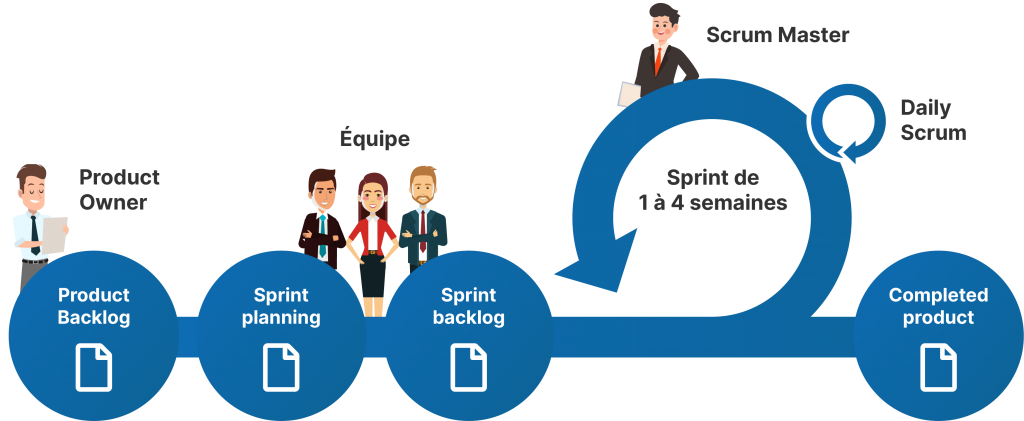
\includegraphics[width=0.8\textwidth]{projet/images/scrum.png}
    \caption{Cycle de vie SCRUM \cite{scrum_guide}}
    \label{fig:scrum_cycle}
\end{figure}

\textbf{Rôles clés :}

\begin{itemize}
    \item \textbf{Product Owner :} Il représente la voix du client au sein de l’équipe. Son rôle consiste à recueillir et analyser les besoins des utilisateurs, puis à les traduire sous forme de User Stories. Il est également responsable de la priorisation des tâches dans le Product Backlog et veille à ce que les fonctionnalités développées répondent aux attentes des utilisateurs.

    \item \textbf{Équipe de développement :} Elle est composée de plusieurs membres chargés de concevoir et réaliser les fonctionnalités définies par le Product Owner. L’équipe est auto-organisée et collaborative, chaque membre contribuant activement à l’atteinte des objectifs du Sprint.

    \item \textbf{Scrum Master :} Il agit comme facilitateur du processus Scrum. Son rôle est de s’assurer de la bonne application des principes Agile, d’aider l’équipe à surmonter les obstacles rencontrés et de garantir le bon déroulement des Sprints afin de maintenir une progression efficace du projet.
\end{itemize}

La méthode Scrum s’appuie également sur des éléments clés appelés artefacts Scrum, qui permettent d’organiser le travail, de suivre l’avancement du projet et d’assurer la transparence au sein de l’équipe.

 
\section{Conclusion}

Ce chapitre constitue une étape primordiale pour fixer les repères de notre projet durant lequel nous avons présenté l’organisme d’accueil et dégagé des attentes du projet après avoir étudié et critiqué l’existant. À la fin, nous avons présenté la méthodologie de travail à utiliser.
 

